% \documentclass[rmp,aps,floatfix,authordate1-4,preprint]{revtex4}
% \documentclass[prb,aps,floatfix,authordate1-4,preprint]{revtex4}

\documentclass[pre,aps,floatfix,authordate1-4,twocolumn]{revtex4-1}
%\documentclass[pre,aps,floatfix,authordate1-4]{revtex4-1}

%\documentclass[aps,prl,preprint,superscriptaddress]{revtex4}



%\documentclass[aps,prl,preprint,groupedaddress]{revtex4}

\usepackage{rotating} 
\usepackage{times}
\usepackage{graphicx}
\usepackage{setspace}
\usepackage{amsmath}
\usepackage{caption}
\usepackage{subcaption}
\usepackage[obeyFinal]{easy-todo}
%\usepackage{scrtime}
\usepackage[multiple]{footmisc}
%\usepackage[sort&compress]{natbib}
%\bibpunct{(}{)}{,}{n}{}{}
%\renewcommand{\bibnumfmt}[1]{#1.}


\begin{document}
%\singlespacing

\title{Towards atomistic resolution structure of phosphatidylcholine glycerol backbone and choline headgroup at different ambient conditions}

%\author{Alexandru Botan}
%
%\author{Andrea Catte}
%\author{Fernando Favela}
\author{Patrick Fuchs}
\thanks{The authors are listed in alphaphetical order.}
\thanks{The author list is not completed.}
\thanks{Institut Jacques Monod, CNRS, Université Paris Diderot, Sorbonne Paris Cité, Paris, France}
%\thanks{Université Paris Diderot, Sorbonne Paris Cité, Paris, France}
%\author{Matti Javanainen}
%\thanks{Tampere University of Technology, Tampere, Finland}
%\author{Waldemar Kulig}
\author{Antti Lamberg}
\thanks{Department of Chemical Engineering, Kyoto University, Kyoto, Japan}
%\author{Alexander Lyubartsev}
\author{Markus S. Miettinen}
\thanks{Fachbereich Physik, Freie Universität Berlin, Berlin, Germany}
%\author{Luca Monticelli}
%\thanks{5IBCP, CNRS UMR 5086, Lyon, France}
%\author{Jukka M\"a\"att\"a}
%\thanks{Aalto University, Espoo, Finland}
%\setcounter{page}{1}
%\author{Vasily Oganesyan}
\author{O. H. Samuli Ollila} 
\thanks{{\bf Author to whom correspondence may be addressed. E-mail: samuli.ollila@aalto.fi.}}
\thanks{Helsinki Biophysics and Biomembrane Group, Department of Biomedical Engineering and Computational Science, Aalto University, Espoo, Finland}
%\author{Marius Retegan}
%\thanks{Max Planck Institute for Chemical Energy Conversion, Mülheim an der Ruhr, Germany}
%\author{Hubert Santuz}
%\thanks{INSERM, U1134, DSIMB; Institut National de la Transfusion Sanguine (INTS); Laboratoire d'Excellence GR-Ex, Paris, France}
%\thanks{Université Paris Diderot, Sorbonne Paris Cité, Paris, France}
%\author{Joona Tynkkynen}
%\author{Mark Wilson}
%\author{Alexander Vogel}



\begin{abstract}
Phospholipids are essential building blocks of biological membranes.
Despite of vast amount of accurate experimental data the atomistic resolution structures sampled by the glycerol backbone and choline headgroup
in phoshatidylcholine bilayers are not known. Atomistic resolution molecular dynamics simulation model 
would automatically resolve the structures giving an interpretation of experimental results, if the model
would reproduce the experimental data. In this work we compare the C-H bond vector order
parameters for glycerol backbone and choline headgroup between 12 different atomistic resolution
models and experiments in fully hydrated lipid bilayer. The current models are not accurately enough to resolve the structure.
However, closer inspection of three best performing models (CHARMM36, GAFFlipid and MacRog) suggest
that improvements in the sampled dihedral angle distributions would potentilly lead to the model which
would resolve the structure. Despite of the inaccuracy in the fully hydrated
structures, the response to the dehydration, i.e. P-N vector tilting more parallel to membrane normal, 
is qualitatively correct in all models. The CHARMM36 and MacRog models describe the interactions
between lipids and cholesterol better than Berger/H\"oltje model.
This work has been, and continues to be, progressed and discussed through the blog: nmrlipids.blogspot.fi. 
Everyone is invited to join the discussion and make contributions through the blog. 
The manuscript will be eventually submitted to an appropriate scientific journal. 
Everyone who has contributed to the work through the blog will be offered 
coauthorship. For more details see: nmrlipids.blogspot.fi. 


\end{abstract}


\maketitle


~\vspace{0.3cm}\\
{\it \bf} 

\section{Introduction}

Phospholipids containing different polar headgroups and different acyl chains are essential building blocks of 
biological membranes. Lamellar phospholipid bilayer structures have been widely studied with various experimental 
and theoretical techniques as a simple model for the biological membranes~\cite{lipowsky95,tieleman97,klauda08,edholm08,tieleman10,piggot12,rabinovich13,marsh13}. 
Phospholipid molecules are composed of hydrophobic acyl chains and hydrophilic headgroup, which are connected by glycerol backbone,
see Fig.~\ref{POPCstructure} for the structure of 1-palmitoyl-2-oleoylphosphatidylcholine (POPC).
The behaviour of the acyl chains in a bilayer is relatively well understood~\cite{Israelachvili80,lipowsky95,tieleman97,klauda08,edholm08,tieleman10,marsh13}. 
The structures sampled by the glycerol backbone and choline, however, are not fully 
resolved since even the most accurate scattering and Nuclear Magnetic Resonance (NMR)
techniques give only a set of values that the structure has to fulfill, but
there is no unique way to derive the actual structure from these parameters~\cite{seelig77b,skarjune79,Israelachvili80,jacobs80,davis83,akutsu91,hong95b,semchyschyn04}.
Several approaches have been used to resolve structural details, but general consensus has not been reached~\cite{seelig77b,skarjune79,Israelachvili80,jacobs80,davis83,akutsu91,hong95b,semchyschyn04}. 
On the other hand, the glycerol backbone structures are similar for various biologically
relevant lipid species (phosphatidylcholine (PC), phosphatidylethanolamine (PE) and phosphatidylglycerol (PG)) 
in various environments~\cite{gally81} and the headgroup choline structures are similar in model membranes and
real cells (mouse fibroblast L-M cell)~\cite{scherer87}.
Thus, the resolvation of phosphatidylcholine glycerol backbone and choline structures would be 
useful for understanding wide range of different biological membranes.

Classical atomistic resolution molecular dynamics simulations have been widely used to study  
lipid bilayers~\cite{tieleman97,klauda08,edholm08,tieleman10,piggot12,rabinovich13}. As these models provide an atomistic
resolution description of the whole lipid molecule, they have potential to resolve the glycerol backbone and 
headgroup structures. In particular, the experimental C-H bond order parameters for the glycerol backbone 
(g$_1$, g$_2$ and g$_3$) and choline ($\alpha$ and $\beta$) segments (see Fig.~\ref{POPCstructure} for definitions) are among the main parameters used in
attempts to derive the structures from experimental data~\cite{seelig77b,skarjune79,jacobs80,davis83,akutsu91,hong95b,semchyschyn04}.
These parameters are also routinely compared between experiments and simulations for the acyl chains~\cite{tieleman97,klauda08,edholm08,tieleman10,piggot12}.
Thus, the structures sampled in a simulation model that reproduces these and other experimental parameters, automatically
give an interpretation of the experiments, in other words they can be considered as reasonable atomistic resolution descriptions of
the behaviour of lipid molecules in a bilayer.

The glycerol backbone and choline headgroup order parameters have been compared between simulations and experiments
in some studies~\cite{hogberg08,castro08,klauda10,kapla12,dickson12,poger12,ferreira13,chowdhary13,maciejewski14}, 
however much less frequently than for acyl tail chains~\cite{tieleman97,klauda08,edholm08,tieleman10,piggot12}.
The main reason is probably that the existing experimental data for the glycerol backbone
and choline headgroups is scattered over many publications and published in a format that is difficult to understand without some NMR expertise. 

In this work we first review the most relevant experimental data for the glycerol backbone and choline headgroup order parameters
in a phosphatidylcholine lipid bilayer. Then the available atomistic resolution lipid models are carefully compared to the 
experimental data. The comparison reveals that the CHARMM36~\cite{klauda10}, GAFFlipid~\cite{dickson12} and MacRog models~\cite{maciejewski14}
have the most realistic glycerol backbone and choline structures. We also compare the glycerol backbone and choline 
structures between the most often used (Berger) lipid model~\cite{berger97} and the best performing models, to demonstrate that by using the 
order parameters we can distinguish the more reasonable structures from the less reasonable ones. However, none of the current models 
is accurate enough to resolve the atomistic resolution stuctures.

In addition to the fully--hydrated single--component lipid bilayers, the glycerol backbone and choline order parameters
have been measured under a large number of different conditions. For example, as a function of hydration level~\cite{bechinger91,ulrich94,dvinskikh05b}, cholesterol content~\cite{brown78,ferreira13}
ion concentration~\cite{brown77,akutsu81,altenbach84,roux90,roux91}, temperature~\cite{gally75}, charged lipid content~\cite{roux90,roux91}, charged surfactant content~\cite{scherer89}, 
drug molecule concentration~\cite{kelusky84,castro08}, and protein content~\cite{roux89,kuchinka89} (listing only the publications most relevant for this work and the pioneering studies).
Awareness of the existence of this type of data allows the comparison of structural responses to varying conditions between simulations and experiments,
which can be used to validate the simulation models and to interpret the original experiments. 
In this publication we demonstrate the power of this approach for understanding the behaviour of a bilayer as a function of hydration level and cholesterol concentration.
Choline headgroup order parameters as function of ion concentration, and their relation to the ion binding affinity, are discussed elsewhere~\cite{ionpaper}.

  \begin{figure}[]
  \centering
  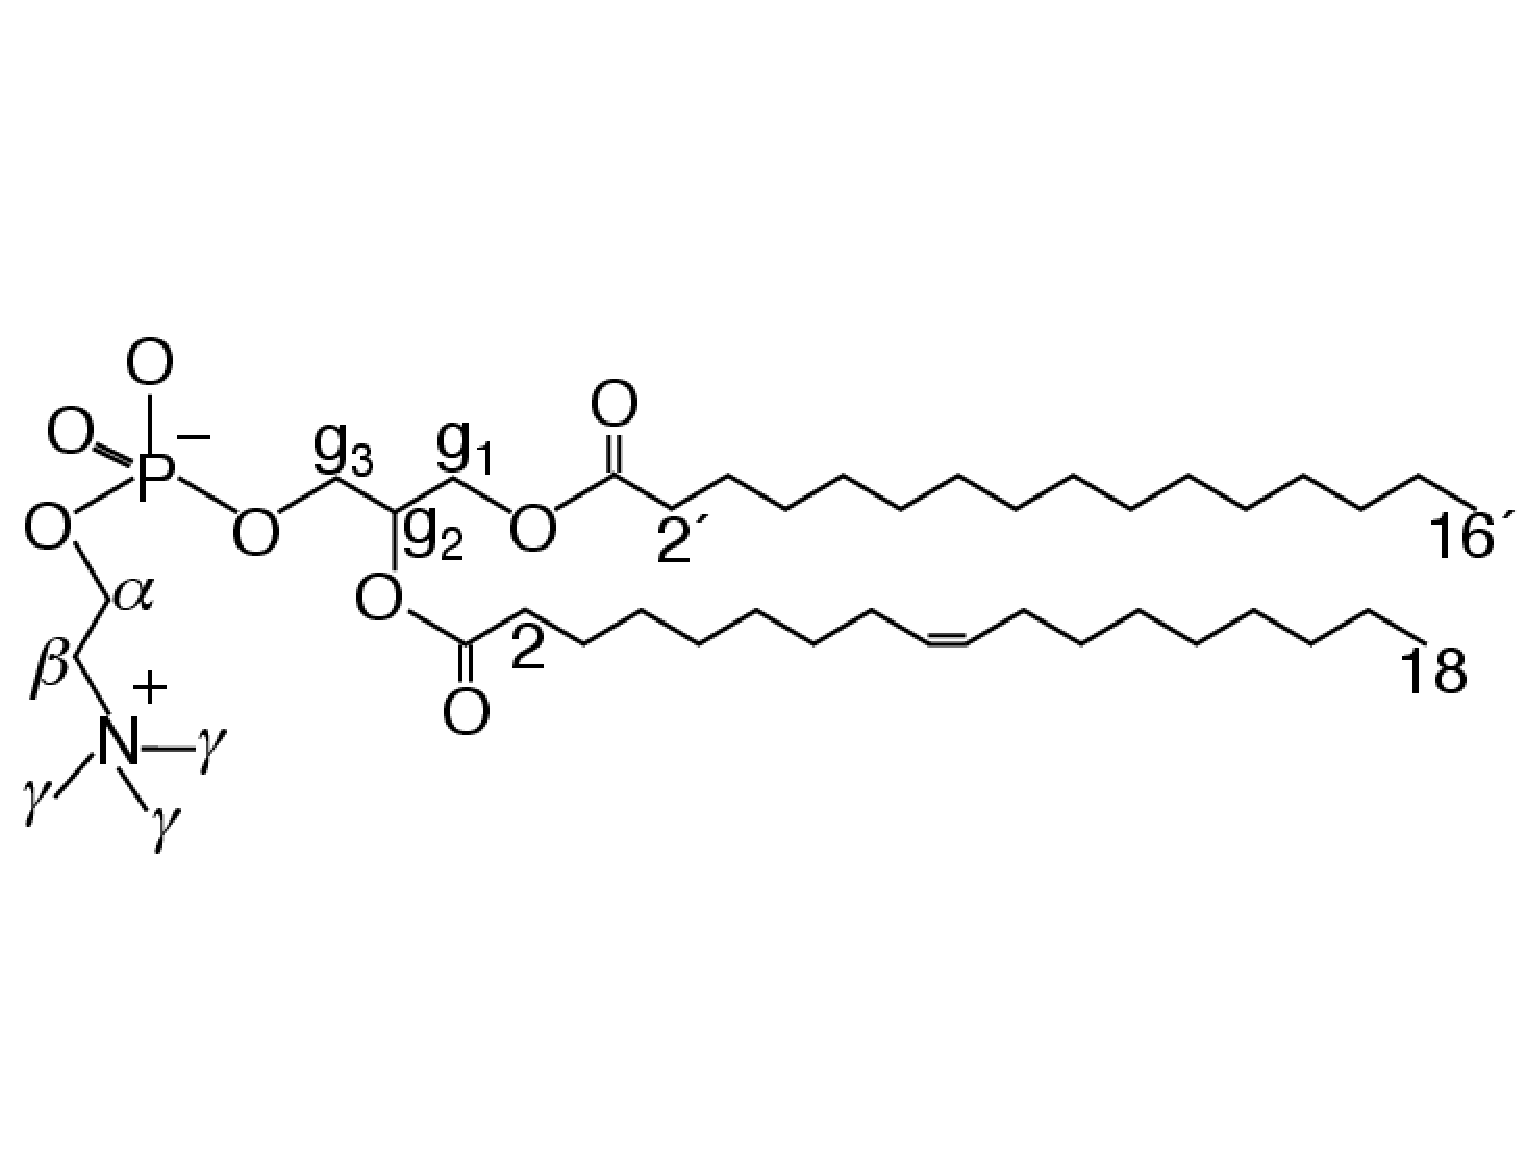
\includegraphics[width=8.6cm]{POPCstructure.eps}

  \caption{\label{POPCstructure}
    Chemical structure of  1-palmitoyl-2-oleoylphosphatidylcholine (POPC).}
  
\end{figure}

\section{methods}

\subsection{Open collaboration}
\todo{How much should we write about this?}

This work has been done, and is continuing, as an open collaboration through nmrlipids.blogspot.fi.

\subsection{Analysis}
The order parameter of a hydrocarbon C-H vector is defined as $S_{{\rm CH}}=\frac{3}{2}\langle \cos^2 \theta-1 \rangle$, where
the average is an ensemble average over the sampled conformations, and $\theta$ is the angle between the C-H bond and the membrane normal.
The order parameters can be measured by detecting quadrupolar splitting with $^2$H NMR~\cite{seelig77c} or by detecting dipolar 
splitting with $^{13}$C NMR~\cite{hong95a,gross97,dvinskikh05a,ferreira13}. The measurements are based on
different physical interactions and also the connection between order parameters and quadrupolar or dipolar splitting
are different. The order parameters from the measured quadrupolar splitting $\Delta \nu_Q$ ($^2$H NMR) are calculated using 
the equation $|S_{{\rm CD}}|=\frac{4}{3} \frac{e^2qQ}{h} \Delta \nu_Q$, where the value for the static quadrupole
splitting constant is estimated from various experiments to be 170~kHz leading to a numerical relation $|S_{{\rm CD}}|=0.00784 \times \Delta \nu_Q$~\cite{seelig77c}. 
The order parameters from the measured dipolar splitting $d_\mathrm{CH}$ ($^{13}$C NMR) are calculated using equation
$|S_{{\rm CH}}|=\frac{4\pi\langle r_\mathrm{CH}^3 \rangle}{\hbar \mu_0 \gamma_h \gamma_c} d_\mathrm{CH}$, where
values between 20.2-22.7 kHz are used for $\frac{4\pi\langle r_\mathrm{CH}^3 \rangle}{\hbar \mu_0 \gamma_h \gamma_c}$,
depending on the original authors~\cite{hong95a,gross97,dvinskikh05a,ferreira13}.
It is important to note that the order parameters measured with different techniques based on different physical interactions are in good agreement
with each other (see Results and Discussion), indicating very high quantitative accuracy of the measurements.
For more detailed discussion see the Supplementary material \todo{The idea is to publish all the blog content as supplementary material or through
Figshare or Zenodo}.

The order parameters from simulations were calculated directly using the definition.
%$S_{{\rm CH}}=\frac{3}{2} \langle \cos^2 \theta-1 \rangle$. 
For the united atom models the hydrogen locations were generated 
post-simulationally using the positions of the heavy atoms in the simulation trajectories.
The statistical error estimates were calculated for the best performing simulation
models by calculating the error of the mean for the average over individual lipids in the system. 





\subsection{Simulated systems}
All simulations are ran with a standard setup for planar lipid bilayer in zero tension
with periodic boundary conditions with Gromacs software package (version numbers ?-? \todo{Data contributors: please deliver the version number you have used}).
The number of molecules, temperatures and the length of simulations for all the fully 
hydrated lipid bilayer simulations are listed in Table~\ref{systems}. Full simulation
details for all simulations are given the next section.

\begin{table*}[htb]
\centering
\caption{Simulated pure lipid bilayers with full hydration.
}\label{systems}
\begin{tabular}{c c c c c c c}
%\hline
Force field & lipid  & \footnote{The number of lipid molecules}N$_{\rm l}$   &  \footnote{The number of water molecules}N$_{\rm w}$ & \footnote{Simulation temperature}T (K)  & \footnote{The total simulation time}t$_{{\rm sim}}$(ns) \todoi{Do we need this or would it be enough to write into the text that "All the simulations were sufficinetly equlibrated before the analysis"?} & \footnote{Time frames used in the analysis}t$_{{\rm anal}}$ (ns)\\
\hline
Berger\cite{berger97}          &   POPC & 128 & 7290  & 298  & 270 & 240  \\
Berger\cite{berger97}          &   POPC & 128 & 7290  & 323  & 56 & 56  \\
Berger\cite{berger97}\todoi{Jukka Maatta, please check the information and deliver missing numbers}          &   DPPC & 72 & ?  & 323  & ? & 100  \\
Berger\cite{berger97}          &   DMPC & 128 & 5097  & 323  & ? & 100  \\
CHARMM36\cite{klauda10}        & POPC   & 72  &  2242 & 303 & 30 & 20  \\
CHARMM36\cite{klauda10}\todoi{Hubert Santuz, please check the information and deliver missing numbers}        & POPC   & 128 &  ?    & 303 & 150 & 50  \\
CHARMM36\cite{klauda10}        & DPPC   & 72  &  2189 & 323 & 30 & 25  \\
CHARMM36\cite{klauda10}\todoi{Hubert Santuz, please check the information and deliver missing numbers}        & DOPC   & 128 &  ?    & 303 & 150 & 50  \\
MacRog\cite{maciejewski14}\todoi{Matti Javanainen, please check the information and deliver missing numbers}  & POPC & 288  & ? & 310 & 100 & 80  \\
GAFFlipid\cite{dickson12}       & POPC & 126  & 3948  & 303 & 137 & 32  \\
Lipid14\cite{dickson14}         & POPC  & 72 & 2234 & 303 & 100 & 50  \\
Poger\cite{poger10}\todoi{Patrick Fuchs, please check the information and deliver missing numbers}             & POPC  &  &  & & &  \\
Slipid\cite{jambeck12}\todoi{Jukka Maatta, please check the information and deliver missing numbers}          & DPPC & ? & ? & ? & ? & 30?  \\
Kukol\cite{kukol09} \todoi{Matti Javanainen, please check the information and deliver missing numbers}         & ?   & ? & ? & ? & ? & ?  \\
Chiu et al.\cite{chiu09}     & POPC  & 128 & 3552  & 298 & 56 & 50 \\
H\"ogberg et al.\cite{hogberg08}\todoi{Alexander Lyubartsev, please check the information and deliver missing numbers}  & POPC   &  ? & ?  & 303 & ? & ?  \\
H\"ogberg et al.\cite{hogberg08}\todoi{Alexander Lyubartsev, please check the information and deliver missing numbers}  & DMPC   &  ? & ?  & 303 & ? & ?  \\
Ulmschneider\cite{Ulmschneider09}\todoi{Matti Javanainen, please check the information and deliver missing numbers}    & POPC  & 128 & ? & 310 & 100 & 50 \\
Tj\"ornhammar et al.\cite{tjornhammar14}\todoi{Matti Javanainen, please check the information and deliver missing numbers}    & DPPC  & 144 & ? & ? & 200 & 100 \\
OPLS-AA\cite{rog09b}\todoi{We have this only with 150mM of NaCl delivered by Joona Tynkkynen. Options are to remove these results from this publicatio, run the simulations without ions (if not yet available), 
  or include the results with ions. In my understanding this is a proto version of MacRog so it could be left out as well. However, for historical reasons and 
to understand literature it might be useful to include also these results.}         &   &  &  & & &  \\
CHARMM36-UA~\cite{henin08,lee14}\todo{Alexandru Botan}     & DLPC   & 128  & ?  & 323 & ? & 20? \\
\end{tabular}
\end{table*} 

The initial structures for the simulations in low hydrated conditions are made by removing the
water molecules from the fully hydrated system to achieve the targeted hydration conditions.



The results for the POPC/cholesterol systems with the Berger lipid~\cite{berger97} and H\"oltje
cholesterol model~\cite{holtje01} were taken directly from Ref.~\cite{ferreira13}.
For the initial structure of CHARMM36-~\cite{klauda10,lim12} and MacRog-~\cite{maciejewski14,kulig14} simulations with cholesterol,
the required amount of lipid molecules were replaced with cholesterol \todo{Contributors: Is this correct?}. 


\subsection{Simulation details} 
\todo{Markus Miettinen suggested that maybe these should be put as a table?} \\
\todo{I think that the mdp files should be preferably shared in addition of writing the details here.}
\subsubsection{Berger}


The Berger force field was used for the POPC~\cite{berger97}, with the dihedral potential next to the double bond 
taken from~\cite{bachar04}. The simulations are identical to previous publications~\cite{ollila07a,ferreira13,ferreira14b}.
Timestep of 2~fs was used with leap-frog integrator. Covalent bond lengths were constrained with LINCS algorithm~\cite{hess97,hess07}. 
Coordinates were written every 10~ps. PME with real space cut-off at 1.0~nm was used 
for electrostatics. Plain cut-off was used for the Lennard-Jones interactions with a 1.0~nm cut-off.
The neighbour lists were updated every 5th step with cut-off at 1.0~nm. Temperature was coupled separately
for lipids and water to 298~K with the velocity-rescale method~\cite{bussi07} with coupling constant 0.1~ps$^{-1}$.
Pressure was semi-isotropically coupled to the atmospheric pressure with the Berendsen method~\cite{berendsen84}.

\subsubsection{CHARMM36}
\todo{Markus Miettinen made the files.}

Timestep of 1~fs was used with leap-frog integrator. Covalent bonds with hydrogens were constrained with LINCS algorithm~\cite{hess97,hess07}. 
Coordinates were written every 5~ps. PME with real space cut-off at 1.4~nm was used 
for electrostatics. Lennard-Jones interactions were switched to zero between 0.8~nm and 1.2~nm.
The neighbour lists were updated every 5th step with cut-off 1.4~nm. Temperature was coupled separately
for lipids and water to 303~K with the velocity-rescale method~\cite{bussi07} with coupling constant 0.2~ps$^{-1}$.
Pressure was semi-isotropically coupled to the atmospheric pressure with the Berendsen method~\cite{berendsen84}.

\todo{Hubert Santuz made the simulations with cholesterol.}

\subsubsection{MacRog}
\todo{Matti Javanainen}
\subsubsection{GAFFLipid}
\todo{Marius Retegan made the files}
The initial structure in Lipidbook had different glycerol backbone isomers in different leaflets. 
To generate the initial structure we took the structure delivered by Slipid developers. Also this strucutre
had on lipid with different glycerol bakcbone isomer. This lipid and one lipid from opposite leaflet were removed
after the system was equilibrated.

Timestep of 2~fs was used in Langevin dynamics with zero friction term and collision frequency of 1.0~ps$^{-1}$. 
Covalent bonds with hydrogens were constrained with LINCS algorithm~\cite{hess97,hess07}.
Coordinates were written every 10~ps. PME with real space cut-off at 1.0~nm was used 
for electrostatics. Plain cut-off with 1~nm was used for Lennardt-Jones interactions. 
The neighbour lists were updated every 5th step with cut-off 1.0~nm. 
Pressure was semi-isotropically coupled to the 1~bar pressure with the Berendsen method~\cite{berendsen84}.
\subsubsection{Lipid14}
\todo{Marius Retegan made the files}

Timestep of 2~fs was used in Langevin dynamics with zero friction term and collision frequency of 1.0~ps$^{-1}$. 
Covalent bonds with hydrogens were constrained with LINCS algorithm~\cite{hess97,hess07}.
Coordinates were written every 10~ps. PME with real space cut-off at 1.0~nm was used 
for electrostatics. Plain cut-off with 1~nm was used for Lennardt-Jones interactions. Dispersion correction
was used for energy and pressure. The neighbour lists were updated every 5th step with cut-off 1.0~nm. 
Pressure was semi-isotropically coupled to the 1~bar pressure with the Berendsen method~\cite{berendsen84}.

\subsubsection{Poger et al.}
\todo{Patrick Fuchs, maybe we should shortly mention the Gromacs version issue here?}
\subsubsection{Slipid}
\todo{Matti Javanainen}
\subsubsection{Kukol}
\todo{Matti Javanainen}
\subsubsection{Chiu et al.}
The force field parameters and the initial configuration were downloaded from: \todo{The page I used does not exist anymore}.
Timestep of 2~fs was used with leap-frog integrator. Covalent bond lengths were constrained with LINCS algorithm~\cite{hess97,hess07}. 
Coordinates were written every 10~ps. PME with real space cut-off at 1.0~nm was used 
for electrostatics. Twin range cut-off was used for the Lennardt-Jones interactions with short and long cut-offs at 1.0~nm and 1.6~nm, respectively.
The neighbour lists were updated every 5th step with cut-off at 1.0~nm. Temperature was coupled separately
for lipids and water to 298~K with the velocity-rescale method~\cite{bussi07} with coupling constant 0.2~ps$^{-1}$.
Pressure was semi-isotropically coupled to the atmospheric pressure with the Parrinello-Rahman method~\cite{parrinello81}.
\subsubsection{H\"ogberg et al.}
\todo{Alexander Luybartsev}
\subsubsection{Ulmschneider}
\todo{Matti Javanainen}
\subsubsection{OPLS-AA}
\todo{Joona Tynkkynen. We have this only with 150mM of NaCl delivered by Joona Tynkkynen. Options are to remove these results from this publicatio, run the simulations without ions (if not yet available), 
  or include the results with ions. In my understanding this is a proto version of MacRog so it could be left out as well. However, for historical reasons and 
to understand literature it might be useful to include also these results.}


\section{Results and Discussion}

\subsection{Full hydration: Experimental order parameters for glycerol backbone and headgroup}\label{experiments}
The specific deuteration of $\alpha$-, $\beta$- and g$_3$- segments of dipalmitoylphosphatidylcholine (DPPC) has been successful, 
allowing the order parameter measurements for these segments by $^2$H--NMR~\cite{gally75,brown77,brown78,akutsu81}.
In addition, the order parameters for all glycerol backbone and choline headgroup segments in egg yolk lecithin~\cite{hong95a},
1,2-dimyristoyl-sn-glycero-3-phosphocholine (DMPC)~\cite{hong95b,gross97,dvinskikh05a}, 
1,2-dioleoyl-sn-glycero-3-phosphocholine (DOPC)~\cite{warschawski05} and POPC~\cite{warschawski05,ferreira13}
have been measured with several different implementations of $^{13}$C NMR experiments.
The experimental absolute values of glycerol backbone and choline order parameters from various publications are shown in Fig.~\ref{HGorderparameters}.
\begin{figure}[]
  \centering
  \includegraphics[width=8.6cm]{comparison12.eps}
\todo{Figure should be updated. At least, the recent results from the model by Tjornhammar and Edholm are missing. Also CHARMM-UA results.} \\
\todo{Markus Miettinen suggested that we should consider making one more figure where only experimental data would be shown and that would be discussed in Section~\ref{experiments}}
  \caption{\label{HGorderparameters}
  Order parameteres from simulations and experiments for glycerol and choline groups.
  The experimental values were taken from the following publications: DMPC 303K from \cite{gross97}, DMPC 314K from \cite{dvinskikh05a}, DPPC 310K from \cite{gally75}, 
  DPPC 323K from \cite{akutsu81}, and POPC 298K \cite{ferreira13}.
  The vertical bars shown for some of the computational values are not error bars, but demonstrate that for 
  these systems we had two data sets; the ends of the bars mark the values from the two sets, and the dot marks their measurement-time-weighted average. 
} 
\end{figure}

In general there is a good agreement between the order parameters measured with different experimental NMR techniques: Almost all the 
reported values are inside variation of $\pm$0.02 (which is also the error estimate given by Gross et al.~\cite{gross97}) 
for all fully hydrated PC bilayer, regardless of the variation in their acyl chain composition and the temperature.
Exception are the somewhat lower order parameters sometimes reported having been measured with $^{13}$C--NMR~\cite{hong95a,hong95b,warschawski05}.
These experiments have not seen in Fig.~\ref{HGorderparameters} as the reported error bars are either relatively large~\cite{hong95a,hong95b}, 
or the spectral resolution is quite low and the numerical lineshape simulations have not been used in the analysis~\cite{warschawski05}.
Therefore it is highly likely that these reported lower order parameters are due to lower experimental 
accuracy and that we exclude these values from our discussion. 
Motivated by the high experimental repeatability, we have highlighted in 
Fig.~\ref{HGorderparameters} subjective sweet spots (light blue areas), within which we expect the calculated absolute 
values of order parameters of a well-performing force field to fall.

In addition to the phosphatidylcholine lipids, similar values of the glycerol backbone order parameters have been measured
for phophatidylethanolamine (PE) and phopshatidylglycerol (PG) in E. Coli extract~\cite{gally81},
indicating that the glycerol backbone structure is similar independent of the headgroup chemistry and lipid environment.
Further, choline order parameters measured from mouse fibroblast L-M cell are similar to the ones in model
membranes~\cite{scherer87}.

In addition to the numerical values, an important feature of the glycerol backbone is the 
inequality of order parameters for the two hydrogens attached to the same carbon in g$_1$ and g$_3$ segments,
while the hydrogens in choline $\alpha$ and $\beta$ segments give equal values.
Note that in this work we call the phenomena of inequal order parameters for hydrogens attached to the same carbon as ''forking'' to avoid 
confusion with dipolar and quadrupolar splitting in NMR terminology. Forking is also observed experimentally for the C$_2$ carbon in the sn-2
chain of all phosholipids, and it is known to arise from differently sampled orientations of the two C-H bonds, not from two 
different populations of lipid conformations~\cite{engel81}. The forking in glycerol backbone g$_3$ segment is small ($\approx$ 0.02) 
and some experiments only report the larger or the average value~\cite{akutsu81,ferreira13}. 
In contrast, forking is significant for the glycerol backbone g$_1$ segment, whose lower order parameter is close to zero and the
larger one has absolute values around 0.13-0.15. Forking was studied in detail by Gally et al.~\cite{gally81}, who used E. Coli to 
stereospecifically deuterate the different hydrogens attached to the g$_1$ or g$_3$ groups in PE lipids, and measured the order parameters from the lipid 
extract. This experiment gave the lower order parameter when deuterium was in the S position of g$_1$ or R position for g$_3$.
Since the glycerol backbone order parameters are very similar irrespective of the headgroup chemistry (PC,PE and PG) or lipid 
environment~\cite{gally81}, it is reasonable to assume that the stereospecifity measured for the PE lipids
holds also for the PC lipids.

In Fig.~\ref{HGorderparameters} we have shown the absolute values of order parameters as these are accessible
with both $^2$H NMR and $^{13}$C NMR techniques. However, $^{13}$C NMR techniques allow also the measurement of 
the sign of the order parameter~\cite{hong95a,hong95b,gross97}. The measured sign is negative for almost all the carbons 
discussed in this work, only $\alpha$ is positive~\cite{hong95a,hong95b,gross97}. 

Combining the experimental information of the sign~\cite{hong95a,hong95b,gross97} and the stereospecifity 
measurements~\cite{gally81} with the absolute value measurements from various techniques~\cite{gally75,akutsu81,gross97,dvinskikh05a,ferreira13}
having high quantitative accuracy,
the most detailed experimentally available order parameter information for the glycerol backbone and choline segments of POPC is obtained.
These data are shown in Fig.~\ref{HGorderparameters2}.
\begin{figure*}[]
  \centering
  \includegraphics[width=8.6cm]{HGorderparameters5.eps} \\
  \todo{Markus Miettinen suggested that we should consider ``spreading'' the values similarly to the figure~\ref{HGorderparameters}} \\
  \todo{I think that we should include the error bars from simulations in this figure. I also think that for CHARMM36 in this figure we should use the 
    results delivered by Hubert Santuz \\ 
    (https://github.com/NMRLipids/nmrlipids.blogspot.fi/blob/master/DATAreportediINblog/POPC/CHARMM36-303K\_blogged-15-01-14.dat) \\
    which are from longer simulations than mine \\
    (https://github.com/NMRLipids/nmrlipids.blogspot.fi/blob/master/DATAreportediINblog/POPC/CHARMM36-303K\_blogged-20-11-13.dat). \\
  For this we would need error bars from simulations by Hubert.}
  \caption{\label{HGorderparameters2}
  Order parameteres from simulations with Berger, CHARMM36, GAFFlipid and Macrog force fields together with experimental values for POPC glycerol and choline groups.
  The magnitudes for experimental order parameters are taken from Ferreira et al.~\cite{ferreira13}, the signs are based on the measurements by Hong et al.~\cite{hong95a,hong95b} 
  and Gross et al.~\cite{gross97}, and the R/S labeling is based in the measurements by Gally et al.~\cite{gally81}.
} 
\end{figure*}

\subsection{Full hydration: Comparison between simulation models and experiments}

The order parameters of the glycerol backbone and headgroup calculated from different force fields for various lipids has been 
previously compared to experiments~\cite{hogberg08,castro08,klauda10,kapla12,dickson12,poger12,ferreira13,chowdhary13,maciejewski14}. 
The general conclusion from these works seems to be that the CHARMM based~\cite{hogberg08,klauda10}, GAFFlipid~\cite{dickson12} and
MacRog~\cite{maciejewski14} force fields perform better for the glycerol backbone and headgroup structures than the Gromos based models~\cite{castro08,kapla12,poger12,ferreira13}.
However, none of the studies exploits the full potential of the available experimental data discussed in previous section; the quantitative accuracy, known signs and stereospecific labeling of
the experimental order parameters.

To get a general idea about the quality of the glycerol backbone and choline headgroup structures in different models, we calculated the absolute
values of the order parameters for these parts from twelve \todo{This number may change} different lipid models (Table~\ref{systems}) and 
plotted the results together with experimental values in Fig.~\ref{HGorderparameters}.
Two criteria were used to judge the quality of the model: {\bf forkings} there must not be significant forking in the $\alpha$ and $\beta$ carbons,
there must be only moderate forking in the g$_3$ carbon and there must be significant forking in the g$_1$ carbon, {\bf absolute values}
should be preferably inside to the subjective sweet spots determined from experiments (blue shaded regions in Fig.~\ref{HGorderparameters}).
None of the studied force fields fulfills these criteria, however, three force fields are closer than others: CHARMM36~\cite{klauda10}, MacRog~\cite{maciejewski14} and GAFFlipid~\cite{dickson12}.
The results for each force field in respect to the above criteria are summarized in Table~\ref{??} \todo{This kind of table should be done or not?}.

The top three models (CHARMM36, MacRog and GAFFlipid) together with the most used lipid model (Berger model) 
were subjected to a more careful comparison including the signs and the sterospecific labeling in Fig.~\ref{HGorderparameters2}.
The essential additional information given by this comparison is that the sign of the $\beta$ carbon order parameter is correct only in CHARMM36 model.


\subsection{Full hydration: Atomistic resolution structures in different models}

The results in the previous section revealed significant differences of the glycerol backbone and choline headgroup
order parameters between different molecular dynamics simulation models.
However, it is not straightforward to conclude which kind of structural differences (if any)
between the models the results indicate, because the mapping from the order parameters to the 
structure is not unique. In this section we demonstrate that 1) the differences in order parameters
indicate significantly different structural sampling strongly correlating with the dihedral angles of the related bonds,
and that 2) the comparison between experimental and simulated order parameters can be used to exclude
nonrealistic structural samping in molecular dynamics simulations. The demonstration is done for 
the dihedral angles defined by the g$_3$-g$_2$-g$_1$-O(sn-1) segments in the glycerol backbone and 
the N-$\beta$-$\alpha$-O segments in the headgroup. These dihedrals were chosen for demonstration, because 
significant differences between the models are observed around these segments in Fig.~\ref{HGorderparameters2}.
We note that performing a similar comparison through all the dihedrals in all the 12 \todo{this number may change} models would probably give highly useful
information to improve the accuracy of simulations, however this is beyond the scope of the current report. 

The dihedral angle distributions for the  g$_3$-g$_2$-g$_1$-O(sn-1) dihedral calculated from different models are
shown in Fig.~\ref{dihDISTS}. The distribution is qualitatively different for the Berger model, showing a maximum in 
the gaughe$^+$-conformation (60$^o$) compared to all the other models showing a maximum in the trans-conformation (180$^o$).
The distributions in all the other models have the same general features, the main difference being that the
fraction of configurations in gaughe$^-$-conformation (-60$^o$) is zero for the MacRog, detectable for the CHARMM36 and
equally large to the gaughe$^+$ fraction in GAFFlipid. From the results we conclude that most likely the wrongly sampled
dihedral angle for the g$_2$-g$_1$ bond explains the significant discrepancy to the experimental order parameters
for the g$_1$ segment in the Berger model (Fig.~\ref{HGorderparameters2}).
\begin{figure}[]
  \centering
  \includegraphics[width=8.6cm]{g1-g2_Cdihs.eps}
  \caption{\label{dihDISTS}
    Dihedral angle distributions for g$_3$-g$_2$-g$_1$-O(sn-1) dihedral from different models (POPC bilayer in full hydration).
  } 
\end{figure}

The dihedral angle distribution for the  N-$\beta$-$\alpha$-O dihedral calculated from the same four models is 
shown in Fig.~\ref{dihDISTS2}. Also for this dihedral there are significant differences in the gauche-trans fractions.
The gaughe conformations are dominant in the CHARMM36 while in MacRog there are only trans conformations present.
Interestingly, the probability of the gaughe conformations correlates with the order parameter difference between the $\beta$ and $\alpha$ segments:
the larger the gaughe fraction the larger the order parameter difference. This suggestion together with the results in 
Fig.~\ref{HGorderparameters2} would indicate that the correct gaughe-trans fraction for N-$\beta$-$\alpha$-O dihedral is 
larger than in GAFFlipid but smaller than in CHARMM36. This happens to be quite close to the gaughe-trans fraction in
the Berger model. However, there is significant forking and numerical values are off from the experiments in the Berger
model suggesting that it has some other inaccuracies.
\begin{figure}[]
  \centering
  \includegraphics[width=8.6cm]{a-bDIHS.eps}
  \caption{\label{dihDISTS2}
    Dihedral angle distributions for N-$\beta$-$\alpha$-O dihedral from different models (POPC bilayer in full hydration).
  } 
\end{figure}

The used examples show that the glycerol backbone order parameters reflect the atomistic resolution structure
and that the comparison with experiments allows the assesment of the quality of the suggested structure. We were able to pinpoint
specific problems in the structures in different models and suggest potential improvement strategies.
If the improved atomistic resolution
molecular dynamics simulation model would reproduce the order parameters and other experimental observables (like chemical shift anisotropy)
with experimental accuracy, it would give an interpretation for the atomistic resolution structure of the glycerol backbone and 
choline~\cite{seelig77b,skarjune79,jacobs80,davis83,akutsu91,hong95b,semchyschyn04}. The research along these lines is left, however,
for future studies.


\subsection{Response to dehydration and cholesterol content}
In addition to pure phosphatidylcholine bilayers at full hydration, the choline headgroup order parameters
have been measured under various different conditions~\cite{gally75,brown77,brown78,akutsu81,altenbach84,scherer89,bechinger91,ulrich94,dvinskikh05b,castro08,kapla12,ferreira13}.
Also the order parameters for the glycerol backbone have been measured with $^{13}$C NMR in dehydrated conditions~\cite{dvinskikh05b}, and as a function 
of anesthetics~\cite{castro08} and glycolipids~\cite{kapla12} for DMPC, and as a function of cholesterol 
concentration for POPC~\cite{ferreira13}. Due to the high resolution in the NMR (especially $^2$H NMR) experiments,
even very small order parameter changes resulting from the varying conditions can be measured (see supplementary
material for more detailed discussion \todo{The idea is to publish all the blog content as supplementary material or through
Figshare or Zenodo}.). However, as already discussed above, it is not simple to deduce 
the structural changes from order parameter changes~\cite{akutsu91,semchyschyn04}. Consequently, comparison of the order parameters
between simulations and experiments in different conditions can be used measure the quality of the force field 
in different situations, and, if the quality is good, to potentially interpret the structural changes in experiments.
Here we exemplify such comparison for a lipid bilayer under low hydration levels and mixed with cholesterol. 
The interaction between ions and phosphatidylcholine bilayer is discussed in a separate work~\cite{ionpaper}.


\subsubsection{Phospholipid bilayer with low hydration level}
The experimental order parameters available in the literature~\cite{dvinskikh05b,ulrich94,bechinger91} 
for the glycerol backbone and choline as a function of hydration level are shown in Fig.~\ref{ordPhydr}. 
The independently reported values for choline segments are in good agreement with each other (despite of 
slight differences in temperature and acyl chain composition),
showing increase for both segments with decreasing hydration level. It should be noted that only 
absolute values were measured in the original experiments~\cite{dvinskikh05b,ulrich94,bechinger91}, but
we have included the signs measured separately~\cite{hong95a,hong95b,gross97}. 
Consequently, the $\beta$ order parameter with negative sign actually increases with dehydration 
since the absolute value decreases~\cite{dvinskikh05b,ulrich94,bechinger91}.
Slight decrease for the glycerol backbone g$_3$- and g$_2$- order parameters were observed with dehydration, 
while g$_1$ remained practically unchanged~\cite{dvinskikh05b}.
\begin{figure}[]
  \centering
  \includegraphics[width=8.6cm]{OrderParameterDEHYDpresentation.eps}
\todo{Markus Miettinen suggested that this plot should be clarified.}
  \caption{\label{ordPhydr}
    The effect of dehydration on glycerol and choline order parameters in experiments.
    The magnitudes of order parameters are measured for DMPC ($^{13}$C NMR) at 314~K~\cite{dvinskikh05b}, 
    for POPC ($^2$H NMR) at 296~K~\cite{bechinger91} and for DOPC ($^2$H NMR) at 303~K~\cite{ulrich94}. 
    The signs are based on the measurements by Hong et al.~\cite{hong95a,hong95b} 
    and Gross et al.~\cite{gross97}.
  }
\end{figure}

Lipid bilayer dehydration has been studied also with molecular dynamics simulations~\cite{mashl01,pertsin05,pertsin07,eun09,eun10,schneck12},
typically motivated by the  discussion about the origin of the ``hydration repulsion''~\cite{israelachvili,israelachvili96,sparr11}.
However, the used simulation models are not typically compared to the experimental choline and glycerol backbone
order parameters (except by Mashl et al.~\cite{mashl01}).
In Fig.~\ref{ordPhydr} the glycerol backbone and choline order parameters as a function of hydration level are shown 
for the CHARMM36, MacRog and GAFFlipid models (having the most realistic atomistic resolution structures) together with the Berger model 
(which is the most used lipid model). The choline order parameters increase with dehydration in all simulation
models, in qualitative agreement with experiments. 
The measured decrease in both g$_3$ and g$_2$ order parameters with dehydration is reproduced only in CHARMM36.

The qualitative agreement with experiments in all simulation models for the $\alpha$ and $\beta$ order parameters  
as a function of hydration indicates that the structural response of the choline headgroup to dehydration is somewhat realistic
despite the unrealistic structures at full hydration. 
The most likely explanation is that the choline group
orients more parallel to the membrane plane with dehydration due to restricted interlamellar space. 
Indeed, the P-N angle vector angle with membrane normal as a function of dehydration shows an increase for
all models as a function of dehydration in Fig.~\ref{PNangle}.
However, the qualitative agreement in the lipid response to dehydration does not guarantee the correct 
free energy landscape if the simulation model has incorrect structure. The influence of this issue to 
dehydration energetics studied with simulations~\cite{eun09,schneck12} is left for future studies.
\begin{figure}[]
  \centering
  \includegraphics[width=8.6cm]{PNangles.eps}

  \caption{\label{PNangle}
    The angle between membrane normal and P-N vector in choline segment as function of
    hydration level calculated from different simulations.
  }
\end{figure}

The response of the glycerol backbone to dehydration seems to be more subtle than of the choline headgroup 
as CHARMM36 is the only model that reproduces the decrease in g$_2$ and g$_3$ segments.


\subsubsection{Phospholipid bilayer mixed with cholesterol}
Phospholipid--cholesterol interactions have been widely studied with theoretical~\cite{huang99,zhu07,rog09,alwarawrah12} and
experimental methods~\cite{brown78,marsh10,ferreira13,marsh13}, since cholesterol is abundant in biological membranes and
it has been suggested to be an important player, for example, in domain formation~\cite{simons04,somerharju09}.
It is widely agreed that cholesterol orders lipid acyl tails thus decreasing the area per molecule (condensing effect),
however, the influence of cholesterol on the lipid headgroup and glycerol backbone are sill debated~\cite{huang99,simons04,somerharju09}.
For example, it has been suggested that the surrounding lipids shield cholesterol from interactions with water by 
tilting their headgroups (``umbrella model'')~\cite{huang99} or that cholesterol acts as a spacer for the headgroups thus increasing 
their entropy and dynamics (``superlattice model'')~\cite{somerharju09}. Both of these suggestions have been supported
by molecular dynamics simulations~\cite{zhu07,alwarawrah12}, and other simulations suggest specific
interactions between the glycerol backbone and cholesterol~\cite{rog09}, however the glycerol backbone and choline headgroup behaviour
as a function of cholesterol content is not compared to experiments in these studies. 

The choline headgroup and glycerol backbone order parameters for POPC measured by $^{13}$C NMR~\cite{ferreira13} and DPPC choline order parameters 
measured by $^{2}$H NMR~\cite{brown78} are shown in Fig.~\ref{ordPchol} as a function of cholesterol content.
The agreement between different experimental results is again very good, showing only very modest changes in 
the choline order parameters as a function of cholesterol content. It should be noted, however, that very small
changes are measurable with high resolution $^{2}$H NMR experiments
and cholesterol causes a measurable increase in the $\beta$ order parameter and a forking in the $\alpha$ order
parameter~\cite{brown78}, but these effects are so small that they are barely visible in the scale used in Fig.~\ref{ordPchol}.
Further, the effects of cholesterol on the glycerol backbone order parameters for POPC from $^{13}$C NMR experiment~\cite{ferreira13} 
is in good agreement with the results for the phosphatidylethanolamine (PE) measured by $^{2}$H NMR~\cite{ghosh82}.
These results further support the idea that the glycerol backbone structural behaviour is independent of the
headgroup composition~\cite{gally81} and that the headgroup stucture is independent of the acyl chain region content unless
charges are present~\cite{scherer87}.
\begin{figure}[]
  \centering
  \includegraphics[width=8.6cm]{OrderParameterCHOLexpVSsim.eps}
  \caption{\label{ordPchol}
    The effect of cholesterol content on the glycerol backbone and choline order parameters in experiments~\cite{brown78,ferreira13} and simulations
    with the Berger/H\"oltje, CHARMM36 and MacRog force fields. The signs in the experimental values are based on the measurements by Hong et al.~\cite{hong95a,hong95b} 
    and Gross et al.~\cite{gross97}.  The most order parameters from Berger/Höltje model for g$_1$ are beoynd the y-axis scale.}
\end{figure}

In addition to the experimental data, the previously published simulation results from the Berger/H\"oltje model~\cite{ferreira13},
and our results from CHARMM36 and MacRog force fields  
are shown in Fig.~\ref{ordPchol}. As already pointed out previosly, the Berger/H\"oltje model
seriously overestimates the effect of cholesterol on the phospholipid glycerol backbone and choline segments~\cite{ferreira13}.
In contrast, the responses of CHARMM36 and MacRog are in better agreement
with experiments. However, in the case of MacRog the possibility of discrepancy with 50 mol-\% of cholesterol
and above cannot be excluded since there is data only up to 40 mol-\% 
\todo{It would be nice to have data also for 50 mol-\% or above with MacRog to get rid of this sentence}. 
CHARMM36 seems to even reproduce the modest changes observed experimentally in glycerol backbone segments 
g$_2$ and g$_3$ with high concetrations of cholesterol \todo{It would be nice to look from CHARMM36 simulations
what happens to the g3 segment (the slight increase of the order parameters as a function of cholesterol)
and see if we could explain it.}.

It should be noted that the CHARMM36 force field parameters (dihedral potentials) for the glycerol backbone have been tuned 
the dihedral potentials to reproduce the correct order parameters at fully hydrated conditions~\cite{klauda10}. 
This procedure contains a risk of overfitting, which would manifest itself as wrong responses to changing conditions. 
According to our results, tuning seems not to lead to overfitting problems in the case of dehydration or lipid-cholesterol mixtures. 



\section{Conclusions}
The atomistic resolution structures sampled by the glycerol backbone and choline headgroup
in phoshatidylcholine bilayers are not known despite of vast amount of accurate experimental
data. Atomistic resolution molecular dynamics simulation model which would reproduce the
experimental data would automatically resolve the structures giving an interpretation of experimental results.
In this work we have collected and reviewed the experimental C-H bond vector order
parameters available in literature. These experimental parameters are then compared to
different atomistic resolution simulation models for fully hydrated bilayer, dehydrated bilayer and
lipid bilayer containing cholesterol. Our results have led to the following conclusions:

- The C-H bond order parameters measured with different NMR techniques are in good agreement
with each others. By combining the experimental results from various sources we concluded
that the order parameters for each C-H bond are known with quantitative accuracy of $\pm$0.02.

- None of the tested models (12 different models  \todo{this number may change}) produces the order parameters with the experimental
accuracy for fully hydrated phoshatidylcholine lipid bilayer. However, the CHARMM36, GAFFlipid and MacRog 
models are relatively close. The structures of these models together with the most used lipid model (Berger) 
were subjected to more careful studies. The results revealed that the current models are not accurate
enough to resolve the atomistic resolution structures sampled by glycerol backbone and choline headgroup.  
However, the correlation between dihedral angle distributions and order parameter differences was found, 
suggesting that careful adjustment of dihedral potentials would potentially lead to the model with correct
structure.

- Independent of the accuracy for fully hydrated lipid bilayer, all the models reproduced the choline response
to the dehydration. This can be explained by the change in the P-N vector tilting more parallel to the membrane
which leads to the increase of order parameters despite of the initial configuration. It should be however noted
that the correct qualitative response do not necessarily indicate correct energetics. 

- The response of glycerol backbone and choline headgroup to the cholesterol content is described more
realistically in CHARMM36 and MacRog models than in the Berger model.

In general, we conclude that the atomistic resolution classical molecular dynamics simulations 
is extremely convenient tool to give structural interpretation for the high resolution NMR data~\cite{ferreira14}. 
However, in the case of phoshatidylcholine glycerol backbone and choline headgroup there is some
further model development required.

This work has been, and continues to be, progressed and discussed through the blog: nmrlipids.blogspot.fi. 
Everyone is invited to join the discussion and make contributions through the blog. 
The manuscript will be eventually submitted to an appropriate scientific journal. 
Everyone who has contributed to the work through the blog will be offered 
coauthorship. For more details see: nmrlipids.blogspot.fi. 



{\bf Acknowledgements: }
OHSO acknowledges Tiago Ferreira and Paavo Kinnunen for useful discussions, the Emil Aaltonen foundation for financial support, Aalto Science-IT project and CSC-IT Center for Science for computational resources. 

\bibliographystyle{apsrev}
\bibliography{refs}

\newpage

\onecolumngrid

 \listoftodos

\end{document}
